\documentclass[a4wide]{report}
\usepackage[utf8]{inputenc}
\usepackage[T1]{fontenc}
\usepackage[portuguese]{babel}
\usepackage{url}
\usepackage{graphicx}
\usepackage[pdf]{graphviz}
\usepackage{hyperref}
\usepackage{xcolor}
\usepackage[a4paper, left=4cm, right=4cm, top=2cm,bottom=2cm]{geometry}
\hypersetup{
    colorlinks=true,
    urlcolor=blue,
    linkcolor=black,
    citecolor=red,
    pdftitle={Relatório de Laboratórios de Informática},
    pdfauthor={Hugo Cruz (a23010), Lino Azevedo (a23015), Dani Cruz (a23016)},
    pdfsubject={Relatório},
    pdfkeywords={Laboratórios, Informática, IPCA}
}
\usepackage{listings}
\lstset{language=C}
\lstset{basicstyle=\small,
        captionpos=b,
        float=tp,
        xleftmargin=-4em,
        xrightmargin=-4em,
        frameround=ttff,
        frame=single,
        floatplacement=tbp}
\def\lstlistlistingname{Listagens de Código}
\def\lstlistingname{Listagem}
\usepackage{amsmath}
\begin{document}
\begin{figure}
\centering
    \vspace{5 cm}
    
\includegraphics[width=0.65\linewidth]{ipcatec.png}
\end{figure}
\title{Relatório de Laboratórios de Informática}
\author{Hugo Cruz (a23010)\\ 
Lino Azevedo (a23015)\\
Dani Cruz (a23016)}
\date{2 de janeiro de 2024}
\maketitle
\begin{abstract} % resumo
Este projeto consiste no desenvolvimento de um programa em C, relacionado com a manipulação de ficheiros CSV , TSV e BIN. Desde início foi nos fornecidos um diretório no github com a uma estrutura de pastas. 
\\
\\
No decorrer deste projeto também utilizamos uma ferramenta de documentação denominada por doxygen, onde foi utilizada para gerar um pdf e uma página html. 
A cerca da nossa \textbf{src/} realizamos a divisão de código em 4 ficheiros principais: sendo esse \textbf{main.c, struct.h, csv.c, tsv.c }, onde desenvolvemos um trabalho coletivo, empenhando-nos  ao máximo para atender as exigências solicitadas. Outro ponto bastante importante na divisão de ficheiros foi a criação de um Makefile, que realiza a compilação de forma automática  com um simples comando. O nosso ficheiro \textit{\textbf{struct.h}} e composto por um conjunto de structs, 
responsáveis por armazenar todas as informações abertas dos ficheiros CSV , TSV e Binários. 
\\
\\
Foi nos solicitados para que o nosso programa admitisse a utilização de ficheiros .bin, onde necessitamos de realizar um programa que se escreve todos os dados de um ficheiro no modo binário.
\\
\\
Por fim desenvolvemos um relatório em latex, sendo algo novo para todos os elementos do grupo, onde se tornou uma experiência enriquecedora para todos os membros, explorando uma nova ferramenta para a apresentação dos resultados do projeto.
\end{abstract}
% ÍNDICES do documento
% índice global:
\tableofcontents
% figuras
\listoffigures
% tabelas
\listoftables
% listagens de código
\lstlistoflistings
\chapter{Introdução}
O presente relatório surge como resultado das atividades desenvolvidas na disciplina de Laboratório de Informática. O principal propósito desta etapa do curso é promover o aprimoramento das habilidades dos alunos no desenvolvimento de projetos práticos utilizando a linguagem de programação C. Este desafio visa não apenas consolidar os conhecimentos teóricos adquiridos ao longo do curso, mas também proporcionar uma oportunidade para aplicar esses conhecimentos, na prática.
\section{Objetivo }
Este projeto tem como principal objetivo aprimorar as nossas habilidades na linguagem de programação C e dominar a manipulação de ficheiros, incluindo formatos como CSV, TSV e BIN. Além disso, visa familiarizar-nos com a ferramenta Doxygen, que desempenha um papel crucial na geração eficiente da documentação do nosso código. Um aspeto fundamental no desenvolvimento deste projeto foi a organização em ficheiros separados (.h e .c) e a criação de um Makefile para automatizar o processo de compilação.
\section{CSV|TSV }
No decorrer deste relatório iremos falar muito sobre ficheiros CSV e TSV, portanto é importante referir o que é um arquivo CSV e TSV. 
CSV - Trata-se de um arquivo de texto que armazena dados em formato tabular, um exemplo muito conhecido é o "excel". Estes ficheiros têm uma particularidade que separa os dados por vírgulas e ponto e virgulas. Visto que o exemplo fornecido no enunciado, era dividido por ponto e virgula optamos pela utilização dos mesmo. 
TSV - Relativamente a ficheiros TSV, tem uma definição parecida, mas em vez de separar os tipos de dados por vírgulas ou pontos e virgulas, utiliza o TAB.
\begin{figure}[h]
\centering
\vspace{0.5cm}
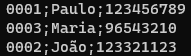
\includegraphics[width=0.3\linewidth]{csv.png}
\hspace{1cm}
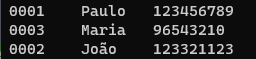
\includegraphics[width=0.3\linewidth]{tsv.png}
\vspace{0.5cm}
\caption{Exemplo de um arquivo CSV | TSV}
\label{fig:csv-label}
\label{fig:tsv-label}
\end{figure}
\chapter{Estrutura do projeto}
Este projeto é composto por dois diretórios principais denominados por: 
\textit{\textbf{\href{https://github.com/LabInf24/d-30-1/tree/main/doc}{/doc}}} - Documentação com o relatório
\textbf{\textit{\href{https://github.com/LabInf24/d-30-1/tree/main/src}{/src}}} - Código da solução desenvolvida
No que diz respeito aos arquivos, todos os documentos localizados no diretório \textit{\textbf{src}} São essenciais para o correto funcionamento deste programa, onde foram separados em ficheiro .c e .h facilitando assim a sua compilação. Quanto ao diretório \textit{\textbf{doc}}, este é constituído por um Doxyfile, fundamental para a geração eficiente da documentação. 
Em seguida vamos abordar um poucos sobre os ficheiros mais relevantes do projeto: 
\subsection{d30/src/main.c} - Trata-se do ficheiro principal, conforme indicado pelo nome, composto pelo nosso main, o qual executa apenas três funções comuns a ficheiros CSV e TSV. Além disso, define o modo de utilização, podendo ser -csv, -tsv, -ajuda e invoca as structs e funções presentes noutros ficheiros denominados csv.c, csv.h, tsv.c e tsv.h.
\subsubsection{Modos}
\begin{lstlisting}[xleftmargin=1em, xrightmargin=1em,language=C, caption={Modo}, label={codigo:c}]
        if (strcmp(argv[1], "-csv") == 0)
        modo = 1;
    else if (strcmp(argv[1], "-tsv") == 0)
        modo = 2;
    else if (strcmp(argv[1], "-ajuda") == 0)
        modo = 3;
    else{
        printf("Caso necessite de ajuda: %s -ajuda\n", argv[0]);
        return 1;
    }\end{lstlisting}
\subsubsection{Função período }
Também implementamos uma função chamada 'período', que pede ao usuário para inserir datas de início e fim (no formato dd-mm) e verifica se as datas estão em intervalos válidos (dia: 1 – 31, mês: 1 – 12). A função persiste na solicitação de entradas até que datas válidas sejam fornecidas.
\begin{table}[h]
    \centering
    \caption{Parâmetros função período} 
    \begin{tabular}{|l|c|} \hline  
         int diainicio& Armazena o dia inicial inserido pelo utilizador \\ \hline  
         int mesinicio& Armazena o mes inicial inserido pelo utilizador \\ \hline  
         int diafim& Armazena o dia final inserido pelo utilizador\\ \hline  
         int mesfim& Armazena o mes final inserido pelo utilizador\\ \hline 
    \end{tabular}
\end{table}
\\
\begin{lstlisting}[language=C, caption={Periodo}, label={codigo:c} , breaklines=true, basicstyle=\small]
void periodo(int *diainicio, int *mesinicio, int *diafim, int *mesfim)
{
    printf("\nDefinir periodo (dd-mm): \n");
    while (*diainicio > 31 || *diainicio < 1 || *mesinicio > 12 || *mesinicio < 1)
    {
        printf("\n\tData de inicio: ");
        scanf("%d-%d", diainicio, mesinicio);
    }

    while (*diafim > 31 || *diafim < 1 || *mesfim > 12 || *mesfim < 1)
    {
        printf("\tData de fim: ");
        scanf("%d-%d", diafim, mesfim);
    }
} 
\end{lstlisting}
\subsubsection{Contador Calorias }
Outra função presente no main é o contador de calorias, esta função solicita ao usuário que insira um valor de calorias (antes de utilizar esta função deve ser usada a função período) e em seguida verifica se a data de cada linha do ficheiro dieta está "dentro" das datas inseridas pelo utilizador.Se tal afirmação se verificar verdadeira e se as calorias do ficheiro dietas forem maiores que as inseridas, realiza a contagem de quantos utilizadores ultrapassaram as calorias (indicadas inicialmente pelo utilizador). Por fim mostra ao utilizador o número de utilizadores que ultrapassam as calorias.
\begin{table}[h]
    \centering
       \caption{Parâmetros função contador calorias} 
    \begin{tabular}{|l|c|}\hline
 Dieta dieta&Invocação da struct Dieta\\\hline  
         int diainicio& Invoca o dia inicial inserido pelo utilizador\\ \hline  
         int mesinicio& Invoca o mes inicial inserido pelo utilizador\\ \hline  
         int diafim& Invoca o dia final inserido pelo utilizador\\ \hline  
         int mesfim& Invoca o mes final inserido pelo utilizador\\ \hline 
    \end{tabular}
\end{table}
\begin{lstlisting}[language=C, caption={Periodo}, label={codigo:c} , breaklines=true, basicstyle=\small]
void contador_calorias(Dieta *dieta, int diainicio, int diafim, int mesinicio, int mesfim){
    float calorias;
    int contador = 0;
    printf("\nDigite o valor de calorias que pretende ver quantos utilizadores ultrapassaram:");
    scanf("%f", &calorias);
    for (int i = 0; i < 4; i++)
    {
        if ((mesinicio < dieta->mes[i] && dieta->mes[i] < mesfim) ||
            (mesinicio == dieta->mes[i] && diainicio <= dieta->dia[i] && dieta->dia[i] <= diafim) ||
            (mesfim == dieta->mes[i] && diainicio <= dieta->dia[i] && dieta->dia[i] <= diafim))
        {
            if (dieta->calorias[i] > calorias)
            {
                contador++;
            }
        }
    }
    printf("\n\tDe 4 utilizadores %d ultrapassaram as %0.01f calorias. \n", contador, calorias);
}
\end{lstlisting}
\subsubsection{Listagem }
Esta função é responsável por ordenar os clientes por ordem decrescente e apresentar os clientes fora do intervalo de calorias.Inicialmente, a mesma verifica se as datas estão em intervalos válidos, restringindo assim alguns dos clientes, caso as datas estejam de fora dos intervalos válidos, compara os números de cliente da struct dieta com os números de cliente da struct plano, garantindo que os clientes que não estão no plano não são apresentados. Por fim, compara as refeições, garantindo que os clientes realizem as refeições planeadas no plano, e valida se estão fora do intervalo de calorias.
\begin{table}[h]
    \centering
       \caption{Parâmetros função listagem} 
    \begin{tabular}{|l|c|}\hline
         Dados dados&Invoca a struct Dados\\ \hline 
         Dieta dieta&Invoca a struct Dieta\\ \hline 
            Plano plano&Invocação da struct Plano\\\hline
         int diainicio& Invoca o dia inicial inserido pelo utilizador\\ \hline  
         int mesinicio& Invoca o mes inicial inserido pelo utilizador\\ \hline  
         int diafim& Invoca o dia final inserido pelo utilizador\\ \hline  
         int mesfim&  Invoca o mes final inserido pelo utilizador\\ \hline 
    \end{tabular} 
\end{table}
\begin{lstlisting}[language=C, caption={Listagem}, label={codigo:c}]
void listagem(Dieta *dieta, Plano *plano, Dados *dados, int diainicio, 
int diafim, int mesinicio, int mesfim)
{
    int j, k, temp;
    int clientes_verificados[4] = {0};
    char nomes_ordenados[max][max];

    for (j = 0; j < 4; j++)
    {
        if ((mesinicio < dieta->mes[j] && dieta->mes[j] < mesfim) 
            ||
            (mesinicio == dieta->mes[j] && diainicio <= dieta->dia[j] 
            && dieta->dia[j] <= diafim) 
            ||
            (mesfim == dieta->mes[j] && diainicio <= dieta->dia[j] 
            && dieta->dia[j] <= diafim))
        {
            for (k = 0; k < 4; k++)
            {
                if (dieta->n_cliente[j] == plano->n_cliente[k])
                {
                    if (strcmp(dieta->refeicao[j], plano->refeicao[k]) == 0)
                    {
                        if (dieta->calorias[j] < plano->calorias_min[k] 
                            || 
                            dieta->calorias[j] > plano->calorias_max[k])
                        {
                            if (dados->n_cliente[j] != 0)
                            {
                                clientes_verificados[j] = dados->n_cliente[j];
                                strcpy(nomes_ordenados[j], dados->nome_cliente[j]);
                            }
                        }
                    }
                }
            }
        }
    }
    for (j = 0; j < 4; j++)
    {
        for (k = j + 1; k < 4; k++)
        {
            if (clientes_verificados[j] < clientes_verificados[k])
            {
                temp = clientes_verificados[j];
                clientes_verificados[j] = clientes_verificados[k];
                clientes_verificados[k] = temp;

                char temp_nome[50];
                strcpy(temp_nome, nomes_ordenados[j]);
                strcpy(nomes_ordenados[j], nomes_ordenados[k]);
                strcpy(nomes_ordenados[k], temp_nome);
            }
        }
    }

    printf("\nListagem dos pacientes ordenada por ordem decrescente:\n\n");
    for (j = 0; j < 4; j++)
    {
        if (clientes_verificados[j] != 0)
        {
            printf("\t%04d %s\n", clientes_verificados[j], nomes_ordenados[j]);
        }
    }
}
\end{lstlisting}
\cite{stackoverflow_sort_structs}
\cite{stackoverflow_sort_strings} 
\begin{figure}[h]
    \centering
    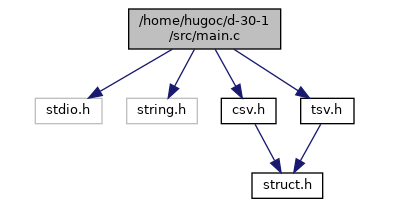
\includegraphics[width=0.8\linewidth]{main.c.png}
    \caption{Divisão do arquivo main.c}
    \label{fig:divisao-tsv}
    \cite{doxygen_manual} 
\end{figure}
\subsection{d30/src/struct.h}
Criamos um arquivo estruturado (struct.h) onde organizamos três entidades fundamentais: a primeira denominada Dados; a segunda designada como Dietas; e, por último, a struct intitulada Planos.
\subsubsection{Dados }
Esta estrutura contém arrays para armazenar o número do cliente, o nome do cliente e o número de telefone associado a cada cliente.
\\
\begin{lstlisting}[xleftmargin=7em, xrightmargin=7em,language=C, caption={Struct Dados}, label={codigo:c}]
typedef struct
{
    int n_cliente[min];
    char nome_cliente[max][max];
    int num_telefone[min];
} Dados;
\end{lstlisting}
\cite{geeksforgeeks_structures} Consultamos esta fonte que foi fundamental para o desenvolvimento do código, fornecendo orientações cruciais. 
\subsubsection{Dieta}
Esta estrutura contém arrays para armazenar o número do cliente, tipos de refeição, tipos de alimento, calorias, e a data de cada refeição.
\\
\begin{lstlisting}[xleftmargin=7em, xrightmargin=7em,language=C, caption={Struct Dieta}, label={codigo:c}]
typedef struct
{
    int n_cliente[min];
    char refeicao[max][max];
    char alimento[max][max];
    int calorias[max];
    int dia[max];
    int mes[max];
    int ano[max];
} Dieta;
\end{lstlisting}
\cite{geeksforgeeks_structures}Ajuda no desenvolvimento das struct
\subsubsection{Plano }
Esta estrutura contém arrays para armazenar o número do cliente, data tipos de refeição, calorias mínimas e máximas.
\\
\begin{lstlisting}[xleftmargin=7em, xrightmargin=7em,language=C, caption={Struct Plano}, label={codigo:c}]
typedef struct
{
    int n_cliente[min];
    int dia[max];
    int mes[max];
    int ano[max];
    char refeicao[max][max];
    int calorias_min[min];
    int calorias_max[min];
} Plano;
\end{lstlisting}
\cite{geeksforgeeks_structures} Consultamos esta fonte que foi fundamental para o desenvolvimento do código, fornecendo orientações cruciais. 
\begin{figure}[h]
    \centering
    \vspace{2 cm}
    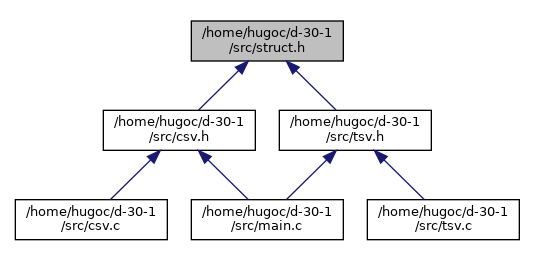
\includegraphics[width=0.8\linewidth]{struct.h.png}
    \caption{Divisão do arquivo struct.h}
    \label{fig:divisaotsv}

\end{figure}
\newpage
\subsection{d30/src/tsv.h}
\begin{lstlisting}[language=C, caption={listar plano tsv}, label={codigo:c}, breaklines=true, basicstyle=\small]
#ifndef TSV_H
#define TSV_H

#include "struct.h"

void ficheiro_tsv_1(char *arquivo, Dados *dados);
void ficheiro_tsv_2(char *arquivo, Dieta *dieta);
void ficheiro_tsv_3(char *arquivo, Plano *plano);
void listar_plano_tsv(Plano *plano, int diainicio, int diafim, int mesinicio, int mesfim);
void calcmedia_tsv(Dados *dados, Dieta *dieta, int diainicio, int mesinicio, int diafim, int mesfim);
void tabela_tsv(Dados *dados, Dieta *dieta, Plano *plano);

#endif
\end{lstlisting}
Até agora, no nosso projeto, completamos algumas etapas iniciais. Começámos por inicializar as funções necessárias e incluir o ficheiro que contém as definições das nossas structs. Essas estruturas serão posteriormente distribuídas pelos ficheiros tsv.c e main.c
\\
\\
\\
\\
\begin{figure}[h]
    \centering
    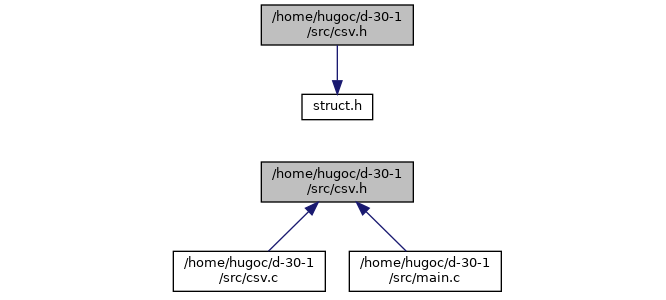
\includegraphics[width=0.8\linewidth]{tsv.h.png}
    \caption{Divisão do arquivo tsv.h}
    \label{fig:divisaotsv}
\end{figure}

\subsection{d30/src/tsv.c}
Na abordagem deste trabalho, utilizamos dois tipos de arquivos: CSV  e TSV. Embora o programa funcione de maneira semelhante para ambos os tipos de arquivos, neste documento, iremos demonstrar as funções implementadas especificamente para o formato TSV. Neste projeto tivemos que realizar a leitura de 3 ficheiros, logo existe 3 funções relativamente ao TSV, mas o raciocínio de desenvolvimento é igual para as 3, logo apenas iremos falar de uma.
\\
\subsubsection{ficheiros tsv 1}
Inicialmente, esta função verifica qual o ficheiro inserido como argumento. Caso seja o permitido, entra no ciclo; caso contrário, apresenta uma mensagem de erro. Relativamente ao ficheiro TSV, efetua a abertura do ficheiro em modo de leitura. Se o ficheiro for nulo, retorna um erro. Em relação à leitura, trata-se de um ciclo while que irá repetir até obter todos os dados, os quais serão armazenados nas nossas structs. Quanto aos ficheiros binários, irá abrir o ficheiro em modo de leitura binária, ler os dados e apresentá-los ao utilizador, armazenando-os também nas nossas structs. 
\begin{table}[h]
    \centering
       \caption{Parâmetros função ficheiro tsv 1} 
    \begin{tabular}{|l|c|}\hline
         Dados dados&Invoca a struct Dados\\ \hline 
         char arquivo&Nome do arquivo TSV a ser lido na função.\\ \hline  
    \end{tabular}
\end{table}
\\

\begin{lstlisting}[language=C, caption={ficheiro tsv 1}, label={codigo:c}]
void ficheiro_tsv_1(char *arquivo, Dados *dados)
{
    if (strcmp(arquivo, "dados.tsv") == 0)
    {
        FILE *ficheiro = fopen(arquivo, "r");

        int i = 0;
        
        if (ficheiro == NULL)
        {
            printf("Erro: N\~ao foi poss\'ivel abrir %s\n", arquivo);
            return;
        }
        printf("\nDados clientes:\n\n");

        while (fscanf(ficheiro, "%d\t%s\t%d\n", &dados->n_cliente[i], 
        dados->nome_cliente[i], &dados->num_telefone[i]) == 3)
        {
            printf("\t%04d %s %d\n", dados->n_cliente[i], 
            dados->nome_cliente[i], dados->num_telefone[i]);
            i++;
        }

        fclose(ficheiro);
    }
    else if (strcmp(arquivo, "dados_tsv.bin") == 0)
    {
        FILE *ficheiro = fopen(arquivo, "rb");
        int i = 0;
        if (ficheiro == NULL)
        {
            printf("Erro: N\~ao foi poss\'ivel abrir o arquivo\n");
            return;
        }
        printf("\nDados clientes:\n\n");

        for (int i = 0; i < 3; i++)
        {
            fread(&dados->n_cliente[i], sizeof(int), 1, ficheiro);
            fread(dados->nome_cliente[i], sizeof(char), max, ficheiro);
            fread(&dados->num_telefone[i], sizeof(int), 1, ficheiro);
        }

        for (int i = 0; i < 3; i++)
        {
            printf("\t%04d %s %d\n", dados->n_cliente[i],  
            dados->nome_cliente[i], dados->num_telefone[i]);
        }

        fclose(ficheiro);
    }
    else
    {
        printf("\nErro: Ficheiro inv\'alido\n");
        return;
    }
}
\end{lstlisting}

\subsubsection{Listar plano tsv}
Criamos como pedido no enunciado uma função que lista o plano nutricional de um paciente para determinada refeição ao longo de um determinado período.
Assim sendo esta função realiza a leitura do número do cliente e da refeição que o utilizador pretende visualizar, verifica o período em seguida compara cliente e refeição com os dados do plano, caso sejam iguais apresenta os dados do cliente caso sejam diferentes não apresenta nada.
\begin{table}[h]
    \centering
    \begin{tabular}{|c|c|} \hline 
         Plano plano& Invoca a struct Planos\\ \hline 
         int diainicio& Invoca o dia inicial inserido pelo utilizador\\ \hline 
         int diafim& Invoca o mes inicial inserido pelo utilizador\\ \hline 
         int mesinicio& Invoca o dia final inserido pelo utilizador\\ \hline 
         int mesfim& Invoca o mes final inserido pelo utilizador\\ \hline
    \end{tabular}
    \caption{Parâmetros função listar plano tsv}
    \label{tab:my_label}
\end{table}
\\
\begin{lstlisting}[language=C, caption={listar plano tsv}, label={codigo:c}, breaklines=true, basicstyle=\small]
void listar_plano_tsv(Plano *plano, int diainicio, int diafim, int mesinicio, int mesfim)
{
    int cliente;
    char refeicao[20];

    printf("\nDigite o cliente e a refeicao que pretende visualizar (numero refeicao):");
    scanf("%d\t %[^\n]", &cliente, refeicao);

    printf("\n\tPlano nutricional do cliente %04d, refeicao:%s\n\n", cliente, refeicao);

    for (int i = 0; i < 100; i++)
    {
        if ((mesinicio < plano->mes[i] && plano->mes[i] < mesfim) ||
            (mesinicio == plano->mes[i] && diainicio <= plano->dia[i] && plano->dia[i] <= diafim) ||
            (mesfim == plano->mes[i] && diainicio <= plano->dia[i] && plano->dia[i] <= diafim))
        {
            if (cliente == plano->n_cliente[i])
            {
                if (strcmp(refeicao, plano->refeicao[i]) == 0)
                {
                    printf("\t%04d %02d-%02d-%d %s %d Cal, %d Cal\n", plano->n_cliente[i], plano->dia[i], plano->mes[i], plano->ano[i], plano->refeicao[i], plano->calorias_min[i], plano->calorias_max[i]);
                }
            }
        }
    }
}
\end{lstlisting}
\newpage
\subsubsection{Calcmedia tsv}
Esta função calcula as médias das calorias consumidas por refeição por cada paciente ao longo de um determinado período.
Começamos por pedir esse período e em seguida verificamos a data em cada linha do ficheiro dieta se esta no período dado pelo utilizador.
Em seguida verificamos qual a refeição em questão (pequeno-almoço, almoço ou jantar) para cada caso se se verificar a condição adicionamos o número de calorias a uma variável própria para essa refeição para o cliente em questão adicionando 1 ao contador para no fim podermos calcular a média.
Por fim se a variável própria que conta as calorias forem diferente de 0 calculamos a média e mostramos ao utilizador.
O exemplo abaixo representa apenas para um cliente sendo que é feito da mesma forma para todos os outros.
\begin{table}[h]
    \centering
    \begin{tabular}{|c|c|} \hline 
          Dados dados& Invoca a struct Dados\\ \hline 
          Dieta dieta& Invoca a struct Dieta\\ \hline 
          Plano plano& Invoca a struct Planos\\ \hline
    \end{tabular}
    \caption{Parâmetros da função tabela tsv}
    \label{tab:my_label}
\end{table}
\begin{lstlisting}[language=C, caption={tabela tsv}, label={codigo:c}, breaklines=true, basicstyle=\small]
void tabela_tsv(Dados *dados, Dieta *dieta, Plano *plano)
{
    float cal_pequeno1 = 0, cal_almoco1 = 0, cal_jantar1 = 0;

    for (int i = 0; i < 6; i++)
    {
        if (dieta->n_cliente[i] == 1)
        {
            if (strcmp(dieta->refeicao[i], "pequeno almoco") == 0)
            {
                cal_pequeno1 += dieta->calorias[i];
            }
            if (strcmp(dieta->refeicao[i], "almoco") == 0)
            {
                cal_almoco1 += dieta->calorias[i];
            }
            if (strcmp(dieta->refeicao[i], "jantar") == 0)
            {
                cal_jantar1 += dieta->calorias[i];
            }
        }
    }

   if (cal_pequeno1 != 0) 
    {
        float media_cal_pequeno1 = cal_pequeno1 / c1_pequeno;                                                  
        printf("\tmedia das calorias consumidas pelo cliente 1 ao pequeno almoco: %.2f\n", media_cal_pequeno1);
    }

    if (cal_almoco1 != 0) 
    {
        float media_cal_almoco1 = cal_almoco1 / c1_almoco;                                            
        printf("\tmedia das calorias consumidas pelo cliente 1 ao almoco: %.2f\n", media_cal_almoco1); 
    }

    if (cal_jantar1 != 0) 
    {
        float media_cal_jantar1 = cal_jantar1 / c1_jantar;                                            
        printf("\tmedia das calorias consumidas pelo cliente 1 ao jantar: %.2f\n", media_cal_jantar1);
    }
}
\end{lstlisting}
\subsubsection{Tabela tsv}
Neste exercício, foi-nos pedido para criar uma tabela do plano nutricional, acumulando as calorias com as mesmas refeições. Inicialmente, realizamos a soma das calorias para cada cliente e para cada refeição. No final, verificamos apenas os números de clientes existentes no plano para evitar trocas de nomes. Certificamo-nos do cliente e da refeição correspondentes, apresentando as linhas da tabela.
\begin{table}[h]
    \centering
    \begin{tabular}{|c|c|} \hline 
          Dados dados& Invoca a struct Dados\\ \hline 
          Dieta dieta& Invoca a struct Dieta\\ \hline 
          Plano plano& Invoca a struct Planos\\ \hline
    \end{tabular}
    \caption{Parâmetros da função tabela tsv}
    \label{tab:my_label}
\end{table}
\begin{lstlisting}[language=C, caption={tabela tsv}, label={codigo:c}, breaklines=true, basicstyle=\small]
void tabela_tsv(Dados *dados, Dieta *dieta, Plano *plano)
{

float cal_pequeno1 = 0, cal_almoco1 = 0, cal_jantar1 = 0;

for (int i = 0; i < 6; i++)
    {
        if (dieta->n_cliente[i] == 1) 
        {
            if (strcmp(dieta->refeicao[i], "pequeno almoco") == 0) 
            {
                cal_pequeno1 = cal_pequeno1 + dieta->calorias[i];
            }
            if (strcmp(dieta->refeicao[i], "almoco") == 0)
            {
                cal_almoco1 = cal_almoco1 + dieta->calorias[i];
            }
            if (strcmp(dieta->refeicao[i], "jantar") == 0) 
            {
                cal_jantar1 = cal_jantar1 + dieta->calorias[i]; 
            }
        }
for (int i = 0; i < 3; i++)
{
    for (int j = 0; j < 3; j++)
    {
        if (dados->n_cliente[i] == plano->n_cliente[j])
        {
            if (dieta->n_cliente[i] == 1)
            {
                if (strcmp(plano->refeicao[j], "jantar") == 0)
                {
                    Apresenta a linha
                }
                else if (strcmp(plano->refeicao[j], "almoco") == 0)
                {
                    Apresenta a linha
                }
                else if (strcmp(plano->refeicao[j], "pequeno almoco") == 0)
                {
                    Apresenta a linha
                }
                else
                {
                    Apresenta a linha
                }
            }
        }
    }
}
\end{lstlisting}
\begin{figure}[h]
    \centering
    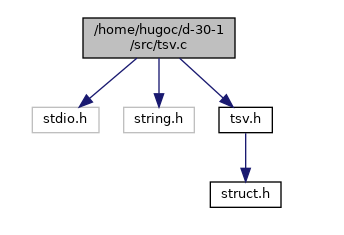
\includegraphics[width=0.5\linewidth]{tsc.c.png}
    \caption{Divisão do arquivo tsv.c}
    \label{fig:divisao-tsv}
 
\end{figure}
\subsection{d30/src/planostsv.bin}
Tivemos a necessidade de desenvolver um código para a criação dos nossos ficheiros binários.
Utilizamos o mesmo método para criar todos eles.
Embora este código não faça parte do trabalho final e, consequentemente, não tenha sido incluído no diretório, desenvolvem-lo para fins de testes e avaliação dos dados.
O método utilizado para a criação dos ficheiros binários segue o seguinte processo:
\\
1. Abrimos o ficheiro em modo de escrita binária ("wb") para garantir que os dados são armazenados em formato binário.
\\
2. Utilizamos a função fwrite para escrever os dados na forma binária no ficheiro.
\\
3. Finalmente, fechamos o ficheiro após a escrita.Este código foi desenvolvido com o objetivo de facilitar o processo de criação de ficheiros binários para fins de teste e não faz parte do produto final do trabalho.
\\
\begin{lstlisting}[language=C, caption={ficheiros binarios}, label={codigo:c}, breaklines=true, basicstyle=\small]
#include <stdio.h>
#include <string.h>
#define max 100
#define min 10
typedef struct
{
    int n_cliente[min];
    int dia[max];
    int mes[max];
    int ano[max];
    char refeicao[max][max];
    int calorias_min[min];
    int calorias_max[min];
} Plano;
int main()
{
    Plano plano;
    FILE *ficheiro = fopen("planos.tsv", "r");
    char linha[100];

    if (ficheiro == NULL)
    {
        printf("Erro: nao foi possivel abrir \n");
        return 1;
    }
    printf("\nPlano nutricional:\n\n");
    
    for (int i = 0; i < 100; i++)
    {
        if (fgets(linha, sizeof(linha), ficheiro) == NULL)
        {
            break;
        }
        sscanf(linha, "%d \t %d-%d-%d \t %99[^\t] \t %d Cal, %d Cal", &plano.n_cliente[i], &plano.dia[i], &plano.mes[i], &plano.ano[i], plano.refeicao[i], &plano.calorias_min[i], &plano.calorias_max[i]);
        printf("\t%04d %02d-%02d-%d %s %d Cal, %d Cal\n", plano.n_cliente[i], plano.dia[i], plano.mes[i], plano.ano[i], plano.refeicao[i], plano.calorias_min[i], plano.calorias_max[i]);
    }
    fclose(ficheiro);

    FILE *ficheiro_bin = fopen("planos_tsv.bin", "wb");

    if (ficheiro_bin == NULL)
    {
        printf("Erro: nao foi possivel abrir o arquivo\n");
        return 1;
    }
    for (int i = 0; i < 3; i++)
    {
        fwrite(&plano.n_cliente[i], sizeof(int), 1, ficheiro_bin);
        fwrite(&plano.dia[i], sizeof(int), 1, ficheiro_bin);
        fwrite(&plano.mes[i], sizeof(int), 1, ficheiro_bin);
        fwrite(&plano.ano[i], sizeof(int), 1, ficheiro_bin);
        fwrite(&plano.refeicao[i], sizeof(char), max, ficheiro);
        fwrite(&plano.calorias_min[i], sizeof(int), 1, ficheiro_bin);
        fwrite(&plano.calorias_max[i], sizeof(int), 1, ficheiro_bin);
    }
    fclose(ficheiro_bin);
}

\end{lstlisting}
\cite{stackoverflow_binary_files} Fonte que nos ajudou a desenvolver este código.
\subsection{d30/src/Makefile}
Na organização de código, onde realizamos a divisão de código em 3 ficheiros, foi nos pedidos para desenvolver um Makefile.  Para compilar este projeto, é necessário ter o comando "make" instalado. Após a instalação, encontrará um ficheiro Makefile no diretório. Este ficheiro é responsável por compilar automaticamente todos os ficheiros. Basta executar o comando make para realizar a compilação.
\\
\begin{lstlisting}[xleftmargin=7em, xrightmargin=7em,language=make, caption={Código Makefile}, label={codigo:makefile}]

all: prog

prog: main.o csv.o tsv.o
        gcc -o prog main.o csv.o tsv.o

main.o: main.c csv.h tsv.h
        gcc -c main.c

csv.o: csv.c csv.h
        gcc -c csv.c

tsv.o: tsv.c tsv.h
        gcc -c tsv.c

clean:
        rm *.o

\end{lstlisting}
\chapter{Decisões Coletivas}
Na nossa colaboração no projeto em grupo, iniciámos o processo com uma seleção criteriosa de ficheiros CSV. Durante a análise, constatámos que esses ficheiros utilizam tanto pontos e vírgulas como vírgulas para delimitar as palavras. 
Essa escolha revelou-se crucial, uma vez que verificámos que as informações no enunciado seguiam precisamente essa estrutura. Assim, decidimos utilizar esses ficheiros para garantir uma correspondência exata com o formato das informações fornecidas, uma conclusão que consideramos a mais apropriada para alcançar os nossos objetivos.
\\
\\
Simultaneamente, ao longo do desenvolvimento do projeto, deparámos-nos com um desafio relacionado à manipulação de variáveis em funções. Após uma ponderação conjunta, optámos por adotar uma abordagem estruturada por meio da utilização de "struct", proporcionando-nos a flexibilidade de utilizar as variáveis em qualquer ponto do código.
\\
\\
Por fim, decidimos ajustar a nossa estratégia em relação aos argumentos. Inicialmente, escolhemos utilizar apenas um argumento para lidar com a possibilidade de problemas relacionados aos ficheiros binários. Posteriormente, expandimos para cinco argumentos, permitindo-nos especificar os ficheiros que desejávamos utilizar.
\section{Estratégia de Desenvolvimento}
-Hugo Cruz (a23010). Implementação do modo de utilização, argumentos, listar o paciente do plano nutricional, tabelas ficheiros binários, e divisão em ficheiros.c .h, CSV, desenvolvimento do relatório.
\\
\\
-Lino Azevedo (a23015): Implementação do contador, listagem de cliente fora intervalo de calorias, calculo da media de calorias por cliente, num determinado período, desenvolvimento do relatório.
\\
\\
-Dani Cruz (a23016). Implementação de ficheiros CSV e TSV, divisão em ficheiros.c .h para as funções TSV, e ficheiro.h contendo as struct, desenvolvimento do relatório.
\\
\chapter{Comando com Sintaxe de Utilização}
Para realizar a execução do programa com ficheiros CSV:
\begin{figure}[h!]
\centering
    
\includegraphics[width=0.5\linewidth]{csvexe.png}
    \caption{CSV}
    \label{fig:divisao-csv}
\end{figure}
\\
Para realizar a execução do programa com ficheiros TSV:
\begin{figure}[h!]
\centering
    
\includegraphics[width=0.5\linewidth]{tsvexe.png}
    \caption{TSV}
    \label{fig:divisao-tsv}
\end{figure}
\\
Para realizar a execução do programa com ficheiros CSV|Bin:
\begin{figure}[h!]
\centering
    
\includegraphics[width=0.5\linewidth]{csvbinexe.png}
    \caption{CSV|Bin}
    \label{fig:divisao-csv-bin}
\end{figure}
\\
Para realizar a execução do programa com ficheiros TSV|Bin:
\begin{figure}[h!]
\centering
    
\includegraphics[width=0.5\linewidth]{tsvbinexe.png}
    \caption{TSV|Bin}
    \label{fig:divisao-tsv-bin}
\end{figure}
\\
\chapter{Conclusão}
O presente relatório é parte integrante da avaliação do trabalho prático da Unidade Curricular Laboratórios de Informática.
\\
\\
Ao longo do projeto, enfrentamos a decisão crucial de não apenas utilizar ficheiros CSV, mas também de incorporar ficheiros TSV, sendo delimitados por tabulações, e posteriormente, ficheiros no formato binário.Durante o desenvolvimento, deparámo-nos com a necessidade de uma abordagem estruturada para manipular variáveis em funções. A decisão coletiva de adotar "struct" conferiu-nos flexibilidade, permitindo o acesso a variáveis em qualquer ponto do código. Esta escolha contribuiu significativamente para a clareza e organização do nosso código.
\\
\\
Uma das etapas que se revelou particularmente desafiadora foi a elaboração do relatório em LaTeX, uma tarefa que conseguimos concluir com êxito.
Este projeto não apenas aprimorou as nossas habilidades técnicas, mas também destacou a importância de decisões ponderadas e flexibilidade durante o processo de desenvolvimento. Cada desafio superado contribuiu para uma compreensão mais profunda das melhores práticas de programação e promoveu um ambiente colaborativo e eficiente na execução do projeto em grupo.
\\
\\
Embora tenha sido uma etapa desafiadora, acreditamos que alcançamos não só os objetivos propostos, mas também os prazos definidos.
\\
\bibliographystyle{plain}
\bibliography{biografia}
\end{document}